% !TEX root = EUDAQUserManual.tex
\section{Introduction}
The EUDAQ software is a data acquisition framework, written in C++,
and designed to be modular and portable, running on Linux, Mac OS X, and Windows.
It was written primarily to run the EUDET-type beam telescope~\cite{Roloff:2009zza,Jansen:2016},
but is designed to be generally useful for other systems.

The hardware-specific parts are kept separate from the core,
so that the core library can still be used independently.
For example, hardware-specific parts are two components for the EUDET-type beam telescope: \gls{TLU} and \gls{NI} for Mimosa 26 sensor read out.

The raw data files generated by the DAQ can be converted to the \gls{LCIO} format,
allowing for analysing the data using the EUTelescope package \cite{eutel2008}.

\subsection{Architecture}
It is split into a number of different processes,
each communicating using TCP/IP sockets (compare \autoref{fig:DAQ}).
A central Run Control provides an interface for controlling the whole DAQ system;
other processes connect to the Run Control to receive commands and to report their status.

\begin{figure}[htb]
  \begin{center}
    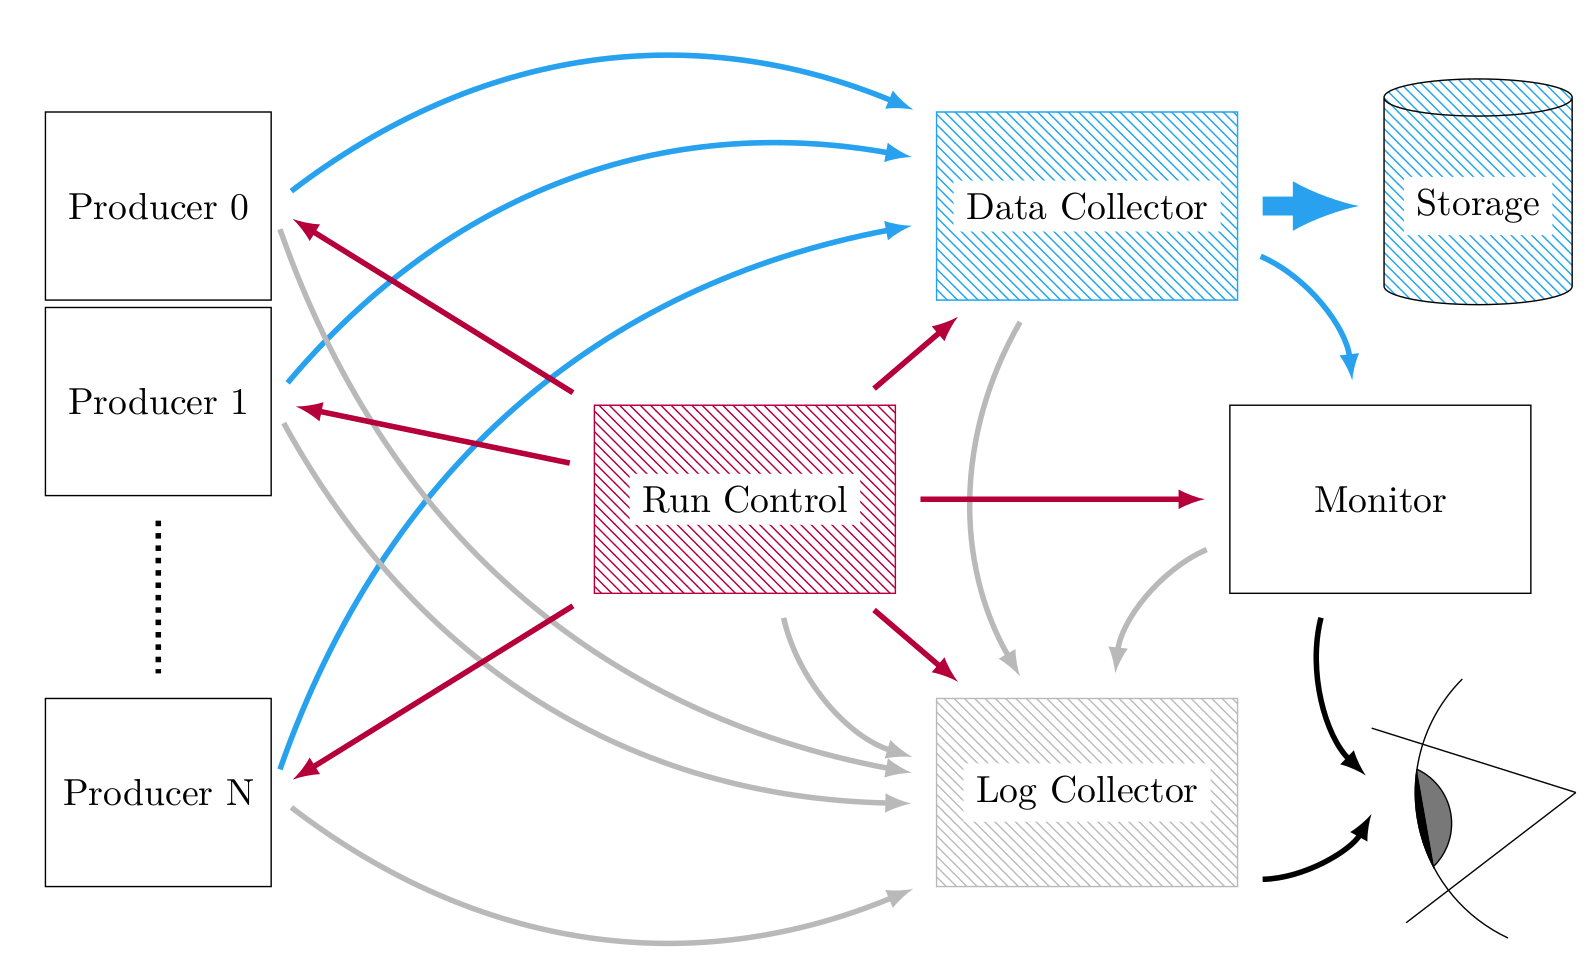
\includegraphics[width=0.9\textwidth]{src/images/eudaq_working_principle}
    \caption{Schematic of the EUDAQ architecture \cite{Spannagel:2017}.}
    \label{fig:DAQ}
  \end{center}
\end{figure}

Each hardware that produces data will have a Producer process (on the left in \autoref{fig:DAQ}).
This will initialize, configure, stop and start the hardware by receiving the commands from the Run Control (red arrows), read out the data and send it to the Data Collector (blue arrows).

The Data Collector receives all the data streams from all the Producers,
and combines them into a single stream that is written to disk (Storage).
It writes the data in a native raw binary format,
but it can be configured to write in other formats, such as \gls{LCIO}.

The Log Collector receives log messages from all other processes (grey arrows),
and displays them to the user, as well as writing them all to file.
This allows for easier debugging, since all log messages are stored together in a central location.

The Monitor reads the data file and generates online-monitoring plots for display.
In the schematic it is shown to communicate with the Data Collector via a socket,
but it actually just reads the data file from disk.

\subsection{Directory and File Structure}
The EUDAQ software is split into several parts that can each be compiled independently,
and are kept in separate subdirectories.
The general structure is outlined below:

\begin{myitemize}
\item \texttt{main}
  contains the core EUDAQ library with the parts that are common to most of the software,
  and several command-line programs that depend only on this library.
  All definitions in the library should be inside the \texttt{eudaq} namespace.
  It is organised into the following subdirectories:
  \begin{myitemize}
  \item \texttt{main/lib/core}
    contains the source code of core library,
  \item \texttt{main/lib/lcio}
    contains the source code of lcio extension library,
  \item \texttt{main/lib/root}
    contains the source code of root extension library,
  \item \texttt{main/module}
    contains the source code of module libraries,
  \item \texttt{main/exe}
    contains the CLI (command line interface) executables source code,
  \end{myitemize}
\item \texttt{gui}
  contains the graphical programs that are built with Qt, such as the RunControl and LogCollector.
\item \texttt{user}
  contains all user provided code shipped with the EUDAQ
  distribution, for example:
  \begin{myitemize}
\item \texttt{user/example}
  contains example code for the intergration with user provides code.
\item \texttt{user/eudet}
  contains the parts that depend on the EUDET-type telescope.
\item e.g. \texttt{user/calice}, \texttt{user/itkstrip}\ldots{}
  contain the code from third-party users.
  \end{myitemize}
\item \texttt{extern}
  global folder which contians external softwares which themselves are not part of EUDAQ project.
\item \texttt{cmake}
  global folder which contians cmake files.
\item \texttt{etc}
  contains configuration files of EUDAQ installation.
\item \texttt{conf}
  contains configuration files for running the beam telescope.
\item \texttt{doc}
  contains source code of documentation, such as this manual.
\end{myitemize}

Each directory containing code has its own \texttt{src} and \texttt{include} subdirectories,
as well as a local \texttt{CMakeLists.txt} and a optional \texttt{cmake} folder containing the rules
for building that directory using \texttt{CMake}.
Header files have a \texttt{.hh} extension so that they can be automatically recognised as C++,
and source files have either \texttt{.cc} for parts of libraries and \texttt{.cxx} for executables.
In the case of any external dependencies are required, there could be a local \texttt{extern} folder

Each directory can contain a \texttt{README.md} file for brief documentation for this specific part, e.g.  
as installation advice. 
Using the \texttt{*.md} file ending allows for applying the Markdown language \cite{markdownWWW}. 
Accordingly, the content will be formatted on the the GitHub platform, where the code is hosted online.
